%!TEX root = ../prueba.tex
En el presente capítulo se realiza la especificación de las máquinas o autómatas finitos que describen:
	\begin{Citemize}
		\item Comportamiento de operaciones sobre actores, términos o entidades de negocio.
		\item Ciclo de Vida de objetos o entidades de negocio.
	\end{Citemize}

Cada máquina de estado tiene una descripción así como los casos de uso asociados a la máquina, también se utiliza un diagrama donde se utiliza la notación U.M.L. para las máquinas de estado.

\begin{Maquina}{MAQMAU01}{Máquina de Estado de la Cuenta de Usuario de una Persona}

\subsection{Resumen}

En cualquier momento dado, la cuenta de un usuario tiene un ’estado’ el  sistema. Las acciones que los actores pueden realizar dependen de dicho estado y pueden tener como consecuencia la transición a otro estado. Los estados y transiciones posibles se muestran en la 	\ref{fig:maqmau01} y se describen a continuación.
	\subsection{Descripción}
	El ciclo de vida de la cuenta de usuario de una  \getElementById[Stakeholder]{Persona} se describe a continuación:
		\begin{description}
			\item[Activo] Este es el estado inicial donde  una persona se registra en el sistema por medio de la aplicación web o la aplicación móvil\footnote{Ver \getElementById[CU]{CUMAU1}} y se le asocia una cuenta de usuario con este estado, el cual permite que la persona acceda a todas las funcionalidades del sistema desde cualquier punto de entrada. Estar en este estado implica:
			
			\begin{Titemize}
			\Titem \getElementById[Stakeholder]{Persona}: 	Este usuario puede: Iniciar sesión en el sistema "Coffee App" por medio de la aplicación web o móvil.
			\end{Titemize}
			
			\item[Bloqueado] Cuando un Usuario con estado \textbf{Activo} ha intentado ingresar al sistema por el control de acceso y se ha equivocado tres veces al ingresar su usuario y/o contraseña, el estado de la cuenta de usuario cambiará a \textbf{Bloqueado}. Estar en este estado implica:
			
			\begin{Titemize}
			\Titem \getElementById[Stakeholder]{Administrador}: 	Este usuario puede: Con base en su criterio, cambiar el estado de la cuenta de usuario a \textbf{Activo}
			\end{Titemize}
			
		\end{description}
	El diagrama correspondiente a la descripción previa se puede observar en la figura \ref{fig:maqmau01}.
	\begin{figure}[hbtp!]
	\begin{center}
		\fbox{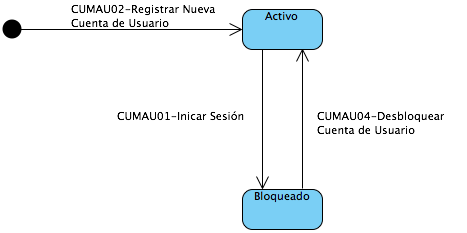
\includegraphics[width=0.7\textwidth]{maquinas/maq-mau01}}
		\caption{Ciclo de Vida de la Cuenta de Usuario de una Persona}
		\label{fig:maqmau01}
		\end{center}
	\end{figure}

\end{Maquina}

\begin{Maquina}{MAQORDEN}{Máquina de Estado de una Orden}
	\subsection{Descripción}
	En cualquier momento dado, una orden tiene un 'estado' en el sistema. Las acciones que los actores pueden realizar sobre una orden dependen de dicho estado y pueden tener como consecuencia la transición a otro estado. Los estados y transiciones posibles se muestran en la figura 	\ref{fig:maqorden} y se describen a continuación.
		\begin{description}
			\item[Confirmado] Es el estado inicial en el que una orden ya ha sido confirmada por un \getElementById[Stakeholder]{Cliente} o una \getElementById[Stakeholder]{Persona} y pasa a la gestión de pedidos de los cocineros para que algún \getElementById[Stakeholder]{Cocinero} pueda comenzar a preparar el pedido, estar en este estado implica que:

		\item \getElementById[Stakeholder]{Cocinero}: Este usuario puede:
		\begin{itemize}
			\item Visualizar la orden y por lo tanto los productos solicitados por un cliente o una persona. 
			\item Comenzar la preparación de la orden. 
		\end{itemize}
		
			\item[Cancelado] Cuando una orden por 
		\end{description}
	\begin{figure}[hbtp!]
	\begin{center}
		\fbox{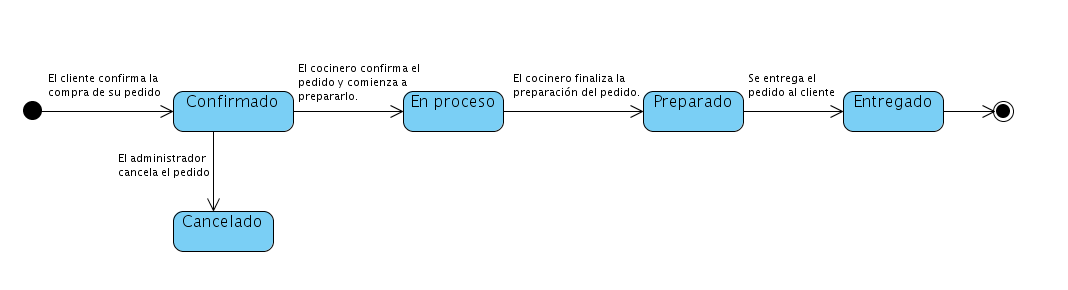
\includegraphics[width=0.7\textwidth]{maquinas/maq-orden}}
		\caption{Ciclo de Vida de una Orden}
		\label{fig:maqorden}
		\end{center}
	\end{figure}

\end{Maquina}


\begin{Maquina}{MAQLOCAL}{Máquina de Estado de un Local}
	\subsection{Descripción}
	En cualquier momento dado, un local tiene un 'estado' en el sistema. Las acciones que se pueden realizar sobre un local dependen de dicho estado y pueden tener como consecuencia la transición a otro estado. Los estados y transiciones posibles se muestran en la figura 	\ref{fig:maqlocal} y se describen a continuación.
			\begin{description}

			\item[Confirmado] Es el estado inicial en el que una orden ya ha sido confirmada por un \getElementById[Stakeholder]{Cliente} o una \getElementById[Stakeholder]{Persona} y pasa a la gestión de pedidos de los cocineros para que algún \getElementById[Stakeholder]{Cocinero} pueda comenzar a preparar el pedido, estar en este estado implica que:
		\item \getElementById[Stakeholder]{Cocinero}: Este usuario puede:
		\begin{itemize}
			\item Visualizar la orden y por lo tanto los productos solicitados por un cliente o una persona. 
			\item Comenzar la preparación de la orden. 
		\end{itemize}
		
			\item[Cancelado] Cuando una orden por 
		\end{description}
	\begin{figure}[hbtp!]
	\begin{center}
		\fbox{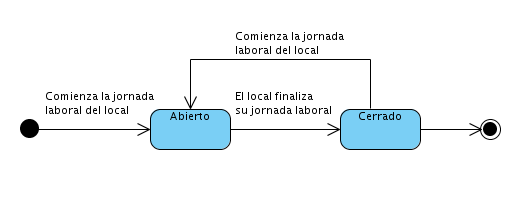
\includegraphics[width=0.7\textwidth]{maquinas/maq-local}}
		\caption{Ciclo de Vida de un Local}
		\label{fig:maqlocal}
		\end{center}
	\end{figure}

\end{Maquina}



\begin{Maquina}{MAQPRODUCTO}{Máquina de Estado de un Producto}
	\subsection{Descripción}
	En cualquier momento dado, un producto tiene un 'estado' en el sistema. Las acciones que se pueden realizar sobre un producto dependen de dicho estado y pueden tener como consecuencia la transición a otro estado. Los estados y transiciones posibles se muestran en la figura 	\ref{fig:maqproducto} y se describen a continuación.
				\begin{description}

			\item[Disponible] Es el estado inicial en el que un producto se encuentra en existencia en un determinado local, estar en este estado implica que:
		\item \getElementById[Stakeholder]{Cliente} o \getElementById[Stakeholder]{Persona}: Los  usuarios pueden:
		\begin{itemize}
			\item Visualizar los productos que esten disponibles.
			\item Agregar al carrito de compras los productos que esten disponibles y que sean de su interes.
						
		\end{itemize}
		
		\item \getElementById[Stakeholder]{Administrador} : El usuario puede:
		\begin{itemize}
			\item Cambiar el estado del producto a \textbf{Agotado}.
						
		\end{itemize}
		
			\item[Agotado] Cuando una orden por 
		\end{description}
	\begin{figure}[hbtp!]
	\begin{center}
		\fbox{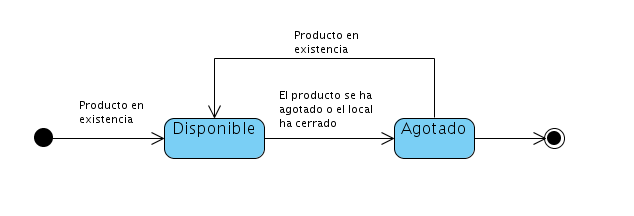
\includegraphics[width=0.7\textwidth]{maquinas/maq-producto}}
		\caption{Ciclo de Vida de un Producto}
		\label{fig:maqproducto}
		\end{center}
	\end{figure}

\end{Maquina}